% Created by tikzDevice version 0.12.3.1 on 2022-08-31 09:40:57
% !TEX encoding = UTF-8 Unicode
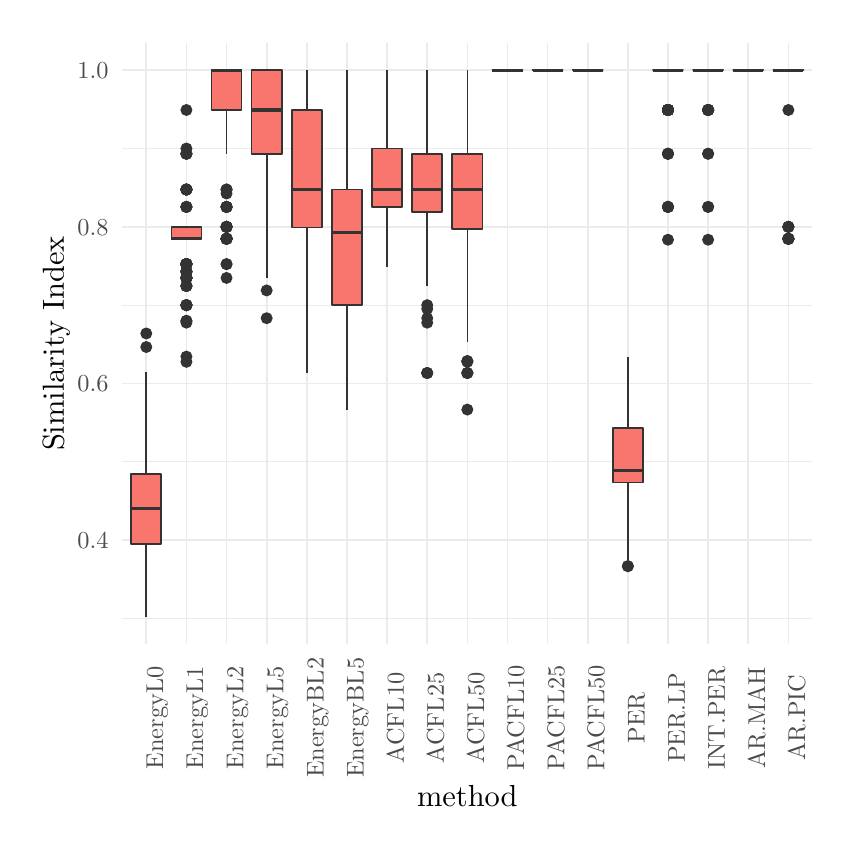
\begin{tikzpicture}[x=1pt,y=1pt]
\definecolor{fillColor}{RGB}{255,255,255}
\path[use as bounding box,fill=fillColor,fill opacity=0.00] (0,0) rectangle (289.08,289.08);
\begin{scope}
\path[clip] ( 34.16, 66.32) rectangle (283.58,283.58);
\definecolor{drawColor}{gray}{0.92}

\path[draw=drawColor,line width= 0.3pt,line join=round] ( 34.16, 75.62) --
	(283.58, 75.62);

\path[draw=drawColor,line width= 0.3pt,line join=round] ( 34.16,132.22) --
	(283.58,132.22);

\path[draw=drawColor,line width= 0.3pt,line join=round] ( 34.16,188.81) --
	(283.58,188.81);

\path[draw=drawColor,line width= 0.3pt,line join=round] ( 34.16,245.41) --
	(283.58,245.41);

\path[draw=drawColor,line width= 0.6pt,line join=round] ( 34.16,103.92) --
	(283.58,103.92);

\path[draw=drawColor,line width= 0.6pt,line join=round] ( 34.16,160.51) --
	(283.58,160.51);

\path[draw=drawColor,line width= 0.6pt,line join=round] ( 34.16,217.11) --
	(283.58,217.11);

\path[draw=drawColor,line width= 0.6pt,line join=round] ( 34.16,273.70) --
	(283.58,273.70);

\path[draw=drawColor,line width= 0.6pt,line join=round] ( 42.86, 66.32) --
	( 42.86,283.58);

\path[draw=drawColor,line width= 0.6pt,line join=round] ( 57.36, 66.32) --
	( 57.36,283.58);

\path[draw=drawColor,line width= 0.6pt,line join=round] ( 71.86, 66.32) --
	( 71.86,283.58);

\path[draw=drawColor,line width= 0.6pt,line join=round] ( 86.36, 66.32) --
	( 86.36,283.58);

\path[draw=drawColor,line width= 0.6pt,line join=round] (100.86, 66.32) --
	(100.86,283.58);

\path[draw=drawColor,line width= 0.6pt,line join=round] (115.36, 66.32) --
	(115.36,283.58);

\path[draw=drawColor,line width= 0.6pt,line join=round] (129.87, 66.32) --
	(129.87,283.58);

\path[draw=drawColor,line width= 0.6pt,line join=round] (144.37, 66.32) --
	(144.37,283.58);

\path[draw=drawColor,line width= 0.6pt,line join=round] (158.87, 66.32) --
	(158.87,283.58);

\path[draw=drawColor,line width= 0.6pt,line join=round] (173.37, 66.32) --
	(173.37,283.58);

\path[draw=drawColor,line width= 0.6pt,line join=round] (187.87, 66.32) --
	(187.87,283.58);

\path[draw=drawColor,line width= 0.6pt,line join=round] (202.37, 66.32) --
	(202.37,283.58);

\path[draw=drawColor,line width= 0.6pt,line join=round] (216.87, 66.32) --
	(216.87,283.58);

\path[draw=drawColor,line width= 0.6pt,line join=round] (231.37, 66.32) --
	(231.37,283.58);

\path[draw=drawColor,line width= 0.6pt,line join=round] (245.88, 66.32) --
	(245.88,283.58);

\path[draw=drawColor,line width= 0.6pt,line join=round] (260.38, 66.32) --
	(260.38,283.58);

\path[draw=drawColor,line width= 0.6pt,line join=round] (274.88, 66.32) --
	(274.88,283.58);
\definecolor{drawColor}{gray}{0.20}
\definecolor{fillColor}{gray}{0.20}

\path[draw=drawColor,line width= 0.4pt,line join=round,line cap=round,fill=fillColor] ( 42.86,178.58) circle (  1.96);

\path[draw=drawColor,line width= 0.4pt,line join=round,line cap=round,fill=fillColor] ( 42.86,173.68) circle (  1.96);

\path[draw=drawColor,line width= 0.6pt,line join=round] ( 42.86,127.74) -- ( 42.86,164.56);

\path[draw=drawColor,line width= 0.6pt,line join=round] ( 42.86,102.62) -- ( 42.86, 76.19);
\definecolor{fillColor}{RGB}{248,118,109}

\path[draw=drawColor,line width= 0.6pt,line join=round,line cap=round,fill=fillColor] ( 37.42,127.74) --
	( 37.42,102.62) --
	( 48.29,102.62) --
	( 48.29,127.74) --
	( 37.42,127.74) --
	cycle;

\path[draw=drawColor,line width= 1.1pt,line join=round] ( 37.42,115.24) -- ( 48.29,115.24);
\definecolor{fillColor}{gray}{0.20}

\path[draw=drawColor,line width= 0.4pt,line join=round,line cap=round,fill=fillColor] ( 57.36,170.22) circle (  1.96);

\path[draw=drawColor,line width= 0.4pt,line join=round,line cap=round,fill=fillColor] ( 57.36,203.63) circle (  1.96);

\path[draw=drawColor,line width= 0.4pt,line join=round,line cap=round,fill=fillColor] ( 57.36,203.63) circle (  1.96);

\path[draw=drawColor,line width= 0.4pt,line join=round,line cap=round,fill=fillColor] ( 57.36,198.65) circle (  1.96);

\path[draw=drawColor,line width= 0.4pt,line join=round,line cap=round,fill=fillColor] ( 57.36,230.58) circle (  1.96);

\path[draw=drawColor,line width= 0.4pt,line join=round,line cap=round,fill=fillColor] ( 57.36,200.94) circle (  1.96);

\path[draw=drawColor,line width= 0.4pt,line join=round,line cap=round,fill=fillColor] ( 57.36,224.31) circle (  1.96);

\path[draw=drawColor,line width= 0.4pt,line join=round,line cap=round,fill=fillColor] ( 57.36,230.58) circle (  1.96);

\path[draw=drawColor,line width= 0.4pt,line join=round,line cap=round,fill=fillColor] ( 57.36,198.65) circle (  1.96);

\path[draw=drawColor,line width= 0.4pt,line join=round,line cap=round,fill=fillColor] ( 57.36,259.33) circle (  1.96);

\path[draw=drawColor,line width= 0.4pt,line join=round,line cap=round,fill=fillColor] ( 57.36,203.63) circle (  1.96);

\path[draw=drawColor,line width= 0.4pt,line join=round,line cap=round,fill=fillColor] ( 57.36,203.63) circle (  1.96);

\path[draw=drawColor,line width= 0.4pt,line join=round,line cap=round,fill=fillColor] ( 57.36,243.52) circle (  1.96);

\path[draw=drawColor,line width= 0.4pt,line join=round,line cap=round,fill=fillColor] ( 57.36,203.63) circle (  1.96);

\path[draw=drawColor,line width= 0.4pt,line join=round,line cap=round,fill=fillColor] ( 57.36,203.63) circle (  1.96);

\path[draw=drawColor,line width= 0.4pt,line join=round,line cap=round,fill=fillColor] ( 57.36,198.65) circle (  1.96);

\path[draw=drawColor,line width= 0.4pt,line join=round,line cap=round,fill=fillColor] ( 57.36,188.81) circle (  1.96);

\path[draw=drawColor,line width= 0.4pt,line join=round,line cap=round,fill=fillColor] ( 57.36,230.58) circle (  1.96);

\path[draw=drawColor,line width= 0.4pt,line join=round,line cap=round,fill=fillColor] ( 57.36,230.58) circle (  1.96);

\path[draw=drawColor,line width= 0.4pt,line join=round,line cap=round,fill=fillColor] ( 57.36,188.81) circle (  1.96);

\path[draw=drawColor,line width= 0.4pt,line join=round,line cap=round,fill=fillColor] ( 57.36,198.65) circle (  1.96);

\path[draw=drawColor,line width= 0.4pt,line join=round,line cap=round,fill=fillColor] ( 57.36,203.63) circle (  1.96);

\path[draw=drawColor,line width= 0.4pt,line join=round,line cap=round,fill=fillColor] ( 57.36,245.41) circle (  1.96);

\path[draw=drawColor,line width= 0.4pt,line join=round,line cap=round,fill=fillColor] ( 57.36,243.52) circle (  1.96);

\path[draw=drawColor,line width= 0.4pt,line join=round,line cap=round,fill=fillColor] ( 57.36,203.63) circle (  1.96);

\path[draw=drawColor,line width= 0.4pt,line join=round,line cap=round,fill=fillColor] ( 57.36,200.94) circle (  1.96);

\path[draw=drawColor,line width= 0.4pt,line join=round,line cap=round,fill=fillColor] ( 57.36,203.63) circle (  1.96);

\path[draw=drawColor,line width= 0.4pt,line join=round,line cap=round,fill=fillColor] ( 57.36,224.31) circle (  1.96);

\path[draw=drawColor,line width= 0.4pt,line join=round,line cap=round,fill=fillColor] ( 57.36,198.65) circle (  1.96);

\path[draw=drawColor,line width= 0.4pt,line join=round,line cap=round,fill=fillColor] ( 57.36,200.94) circle (  1.96);

\path[draw=drawColor,line width= 0.4pt,line join=round,line cap=round,fill=fillColor] ( 57.36,198.65) circle (  1.96);

\path[draw=drawColor,line width= 0.4pt,line join=round,line cap=round,fill=fillColor] ( 57.36,198.65) circle (  1.96);

\path[draw=drawColor,line width= 0.4pt,line join=round,line cap=round,fill=fillColor] ( 57.36,195.73) circle (  1.96);

\path[draw=drawColor,line width= 0.4pt,line join=round,line cap=round,fill=fillColor] ( 57.36,224.31) circle (  1.96);

\path[draw=drawColor,line width= 0.4pt,line join=round,line cap=round,fill=fillColor] ( 57.36,200.94) circle (  1.96);

\path[draw=drawColor,line width= 0.4pt,line join=round,line cap=round,fill=fillColor] ( 57.36,182.48) circle (  1.96);

\path[draw=drawColor,line width= 0.4pt,line join=round,line cap=round,fill=fillColor] ( 57.36,188.81) circle (  1.96);

\path[draw=drawColor,line width= 0.4pt,line join=round,line cap=round,fill=fillColor] ( 57.36,203.63) circle (  1.96);

\path[draw=drawColor,line width= 0.4pt,line join=round,line cap=round,fill=fillColor] ( 57.36,188.81) circle (  1.96);

\path[draw=drawColor,line width= 0.4pt,line join=round,line cap=round,fill=fillColor] ( 57.36,198.65) circle (  1.96);

\path[draw=drawColor,line width= 0.4pt,line join=round,line cap=round,fill=fillColor] ( 57.36,243.52) circle (  1.96);

\path[draw=drawColor,line width= 0.4pt,line join=round,line cap=round,fill=fillColor] ( 57.36,188.81) circle (  1.96);

\path[draw=drawColor,line width= 0.4pt,line join=round,line cap=round,fill=fillColor] ( 57.36,203.63) circle (  1.96);

\path[draw=drawColor,line width= 0.4pt,line join=round,line cap=round,fill=fillColor] ( 57.36,195.73) circle (  1.96);

\path[draw=drawColor,line width= 0.4pt,line join=round,line cap=round,fill=fillColor] ( 57.36,200.94) circle (  1.96);

\path[draw=drawColor,line width= 0.4pt,line join=round,line cap=round,fill=fillColor] ( 57.36,195.73) circle (  1.96);

\path[draw=drawColor,line width= 0.4pt,line join=round,line cap=round,fill=fillColor] ( 57.36,230.58) circle (  1.96);

\path[draw=drawColor,line width= 0.4pt,line join=round,line cap=round,fill=fillColor] ( 57.36,230.58) circle (  1.96);

\path[draw=drawColor,line width= 0.4pt,line join=round,line cap=round,fill=fillColor] ( 57.36,168.33) circle (  1.96);

\path[draw=drawColor,line width= 0.4pt,line join=round,line cap=round,fill=fillColor] ( 57.36,198.65) circle (  1.96);

\path[draw=drawColor,line width= 0.4pt,line join=round,line cap=round,fill=fillColor] ( 57.36,243.52) circle (  1.96);

\path[draw=drawColor,line width= 0.4pt,line join=round,line cap=round,fill=fillColor] ( 57.36,203.63) circle (  1.96);

\path[draw=drawColor,line width= 0.4pt,line join=round,line cap=round,fill=fillColor] ( 57.36,198.65) circle (  1.96);

\path[draw=drawColor,line width= 0.4pt,line join=round,line cap=round,fill=fillColor] ( 57.36,188.81) circle (  1.96);

\path[draw=drawColor,line width= 0.4pt,line join=round,line cap=round,fill=fillColor] ( 57.36,203.63) circle (  1.96);

\path[draw=drawColor,line width= 0.4pt,line join=round,line cap=round,fill=fillColor] ( 57.36,200.94) circle (  1.96);

\path[draw=drawColor,line width= 0.4pt,line join=round,line cap=round,fill=fillColor] ( 57.36,203.63) circle (  1.96);

\path[draw=drawColor,line width= 0.4pt,line join=round,line cap=round,fill=fillColor] ( 57.36,224.31) circle (  1.96);

\path[draw=drawColor,line width= 0.4pt,line join=round,line cap=round,fill=fillColor] ( 57.36,203.63) circle (  1.96);

\path[draw=drawColor,line width= 0.4pt,line join=round,line cap=round,fill=fillColor] ( 57.36,230.58) circle (  1.96);

\path[draw=drawColor,line width= 0.4pt,line join=round,line cap=round,fill=fillColor] ( 57.36,198.65) circle (  1.96);

\path[draw=drawColor,line width= 0.4pt,line join=round,line cap=round,fill=fillColor] ( 57.36,195.73) circle (  1.96);

\path[draw=drawColor,line width= 0.4pt,line join=round,line cap=round,fill=fillColor] ( 57.36,203.63) circle (  1.96);

\path[draw=drawColor,line width= 0.4pt,line join=round,line cap=round,fill=fillColor] ( 57.36,183.15) circle (  1.96);

\path[draw=drawColor,line width= 0.4pt,line join=round,line cap=round,fill=fillColor] ( 57.36,230.58) circle (  1.96);

\path[draw=drawColor,line width= 0.4pt,line join=round,line cap=round,fill=fillColor] ( 57.36,183.15) circle (  1.96);

\path[draw=drawColor,line width= 0.4pt,line join=round,line cap=round,fill=fillColor] ( 57.36,203.63) circle (  1.96);

\path[draw=drawColor,line width= 0.6pt,line join=round] ( 57.36,217.11) -- ( 57.36,217.11);

\path[draw=drawColor,line width= 0.6pt,line join=round] ( 57.36,212.80) -- ( 57.36,212.80);
\definecolor{fillColor}{RGB}{248,118,109}

\path[draw=drawColor,line width= 0.6pt,line join=round,line cap=round,fill=fillColor] ( 51.92,217.11) --
	( 51.92,212.80) --
	( 62.80,212.80) --
	( 62.80,217.11) --
	( 51.92,217.11) --
	cycle;

\path[draw=drawColor,line width= 1.1pt,line join=round] ( 51.92,212.80) -- ( 62.80,212.80);
\definecolor{fillColor}{gray}{0.20}

\path[draw=drawColor,line width= 0.4pt,line join=round,line cap=round,fill=fillColor] ( 71.86,230.58) circle (  1.96);

\path[draw=drawColor,line width= 0.4pt,line join=round,line cap=round,fill=fillColor] ( 71.86,212.80) circle (  1.96);

\path[draw=drawColor,line width= 0.4pt,line join=round,line cap=round,fill=fillColor] ( 71.86,203.63) circle (  1.96);

\path[draw=drawColor,line width= 0.4pt,line join=round,line cap=round,fill=fillColor] ( 71.86,217.11) circle (  1.96);

\path[draw=drawColor,line width= 0.4pt,line join=round,line cap=round,fill=fillColor] ( 71.86,198.65) circle (  1.96);

\path[draw=drawColor,line width= 0.4pt,line join=round,line cap=round,fill=fillColor] ( 71.86,224.31) circle (  1.96);

\path[draw=drawColor,line width= 0.4pt,line join=round,line cap=round,fill=fillColor] ( 71.86,212.80) circle (  1.96);

\path[draw=drawColor,line width= 0.4pt,line join=round,line cap=round,fill=fillColor] ( 71.86,212.80) circle (  1.96);

\path[draw=drawColor,line width= 0.4pt,line join=round,line cap=round,fill=fillColor] ( 71.86,217.11) circle (  1.96);

\path[draw=drawColor,line width= 0.4pt,line join=round,line cap=round,fill=fillColor] ( 71.86,217.11) circle (  1.96);

\path[draw=drawColor,line width= 0.4pt,line join=round,line cap=round,fill=fillColor] ( 71.86,212.80) circle (  1.96);

\path[draw=drawColor,line width= 0.4pt,line join=round,line cap=round,fill=fillColor] ( 71.86,203.63) circle (  1.96);

\path[draw=drawColor,line width= 0.4pt,line join=round,line cap=round,fill=fillColor] ( 71.86,224.31) circle (  1.96);

\path[draw=drawColor,line width= 0.4pt,line join=round,line cap=round,fill=fillColor] ( 71.86,217.11) circle (  1.96);

\path[draw=drawColor,line width= 0.4pt,line join=round,line cap=round,fill=fillColor] ( 71.86,224.31) circle (  1.96);

\path[draw=drawColor,line width= 0.4pt,line join=round,line cap=round,fill=fillColor] ( 71.86,217.11) circle (  1.96);

\path[draw=drawColor,line width= 0.4pt,line join=round,line cap=round,fill=fillColor] ( 71.86,230.58) circle (  1.96);

\path[draw=drawColor,line width= 0.4pt,line join=round,line cap=round,fill=fillColor] ( 71.86,224.31) circle (  1.96);

\path[draw=drawColor,line width= 0.4pt,line join=round,line cap=round,fill=fillColor] ( 71.86,212.80) circle (  1.96);

\path[draw=drawColor,line width= 0.4pt,line join=round,line cap=round,fill=fillColor] ( 71.86,217.11) circle (  1.96);

\path[draw=drawColor,line width= 0.4pt,line join=round,line cap=round,fill=fillColor] ( 71.86,229.15) circle (  1.96);

\path[draw=drawColor,line width= 0.4pt,line join=round,line cap=round,fill=fillColor] ( 71.86,212.80) circle (  1.96);

\path[draw=drawColor,line width= 0.4pt,line join=round,line cap=round,fill=fillColor] ( 71.86,212.80) circle (  1.96);

\path[draw=drawColor,line width= 0.4pt,line join=round,line cap=round,fill=fillColor] ( 71.86,224.31) circle (  1.96);

\path[draw=drawColor,line width= 0.4pt,line join=round,line cap=round,fill=fillColor] ( 71.86,217.11) circle (  1.96);

\path[draw=drawColor,line width= 0.4pt,line join=round,line cap=round,fill=fillColor] ( 71.86,212.80) circle (  1.96);

\path[draw=drawColor,line width= 0.4pt,line join=round,line cap=round,fill=fillColor] ( 71.86,212.80) circle (  1.96);

\path[draw=drawColor,line width= 0.4pt,line join=round,line cap=round,fill=fillColor] ( 71.86,212.80) circle (  1.96);

\path[draw=drawColor,line width= 0.4pt,line join=round,line cap=round,fill=fillColor] ( 71.86,224.31) circle (  1.96);

\path[draw=drawColor,line width= 0.4pt,line join=round,line cap=round,fill=fillColor] ( 71.86,230.58) circle (  1.96);

\path[draw=drawColor,line width= 0.4pt,line join=round,line cap=round,fill=fillColor] ( 71.86,212.80) circle (  1.96);

\path[draw=drawColor,line width= 0.6pt,line join=round] ( 71.86,273.70) -- ( 71.86,273.70);

\path[draw=drawColor,line width= 0.6pt,line join=round] ( 71.86,259.33) -- ( 71.86,243.52);
\definecolor{fillColor}{RGB}{248,118,109}

\path[draw=drawColor,line width= 0.6pt,line join=round,line cap=round,fill=fillColor] ( 66.42,273.70) --
	( 66.42,259.33) --
	( 77.30,259.33) --
	( 77.30,273.70) --
	( 66.42,273.70) --
	cycle;

\path[draw=drawColor,line width= 1.1pt,line join=round] ( 66.42,273.70) -- ( 77.30,273.70);
\definecolor{fillColor}{gray}{0.20}

\path[draw=drawColor,line width= 0.4pt,line join=round,line cap=round,fill=fillColor] ( 86.36,184.10) circle (  1.96);

\path[draw=drawColor,line width= 0.4pt,line join=round,line cap=round,fill=fillColor] ( 86.36,194.13) circle (  1.96);

\path[draw=drawColor,line width= 0.6pt,line join=round] ( 86.36,273.70) -- ( 86.36,273.70);

\path[draw=drawColor,line width= 0.6pt,line join=round] ( 86.36,243.52) -- ( 86.36,198.65);
\definecolor{fillColor}{RGB}{248,118,109}

\path[draw=drawColor,line width= 0.6pt,line join=round,line cap=round,fill=fillColor] ( 80.92,273.70) --
	( 80.92,243.52) --
	( 91.80,243.52) --
	( 91.80,273.70) --
	( 80.92,273.70) --
	cycle;

\path[draw=drawColor,line width= 1.1pt,line join=round] ( 80.92,259.33) -- ( 91.80,259.33);

\path[draw=drawColor,line width= 0.6pt,line join=round] (100.86,259.33) -- (100.86,273.70);

\path[draw=drawColor,line width= 0.6pt,line join=round] (100.86,216.89) -- (100.86,164.29);

\path[draw=drawColor,line width= 0.6pt,line join=round,line cap=round,fill=fillColor] ( 95.42,259.33) --
	( 95.42,216.89) --
	(106.30,216.89) --
	(106.30,259.33) --
	( 95.42,259.33) --
	cycle;

\path[draw=drawColor,line width= 1.1pt,line join=round] ( 95.42,230.58) -- (106.30,230.58);

\path[draw=drawColor,line width= 0.6pt,line join=round] (115.36,230.58) -- (115.36,273.70);

\path[draw=drawColor,line width= 0.6pt,line join=round] (115.36,188.81) -- (115.36,151.08);

\path[draw=drawColor,line width= 0.6pt,line join=round,line cap=round,fill=fillColor] (109.93,230.58) --
	(109.93,188.81) --
	(120.80,188.81) --
	(120.80,230.58) --
	(109.93,230.58) --
	cycle;

\path[draw=drawColor,line width= 1.1pt,line join=round] (109.93,215.22) -- (120.80,215.22);

\path[draw=drawColor,line width= 0.6pt,line join=round] (129.87,245.41) -- (129.87,273.70);

\path[draw=drawColor,line width= 0.6pt,line join=round] (129.87,224.31) -- (129.87,202.74);

\path[draw=drawColor,line width= 0.6pt,line join=round,line cap=round,fill=fillColor] (124.43,245.41) --
	(124.43,224.31) --
	(135.30,224.31) --
	(135.30,245.41) --
	(124.43,245.41) --
	cycle;

\path[draw=drawColor,line width= 1.1pt,line join=round] (124.43,230.58) -- (135.30,230.58);
\definecolor{fillColor}{gray}{0.20}

\path[draw=drawColor,line width= 0.4pt,line join=round,line cap=round,fill=fillColor] (144.37,187.46) circle (  1.96);

\path[draw=drawColor,line width= 0.4pt,line join=round,line cap=round,fill=fillColor] (144.37,188.81) circle (  1.96);

\path[draw=drawColor,line width= 0.4pt,line join=round,line cap=round,fill=fillColor] (144.37,164.29) circle (  1.96);

\path[draw=drawColor,line width= 0.4pt,line join=round,line cap=round,fill=fillColor] (144.37,164.29) circle (  1.96);

\path[draw=drawColor,line width= 0.4pt,line join=round,line cap=round,fill=fillColor] (144.37,182.48) circle (  1.96);

\path[draw=drawColor,line width= 0.4pt,line join=round,line cap=round,fill=fillColor] (144.37,164.29) circle (  1.96);

\path[draw=drawColor,line width= 0.4pt,line join=round,line cap=round,fill=fillColor] (144.37,184.10) circle (  1.96);

\path[draw=drawColor,line width= 0.6pt,line join=round] (144.37,243.52) -- (144.37,273.70);

\path[draw=drawColor,line width= 0.6pt,line join=round] (144.37,222.51) -- (144.37,195.73);
\definecolor{fillColor}{RGB}{248,118,109}

\path[draw=drawColor,line width= 0.6pt,line join=round,line cap=round,fill=fillColor] (138.93,243.52) --
	(138.93,222.51) --
	(149.80,222.51) --
	(149.80,243.52) --
	(138.93,243.52) --
	cycle;

\path[draw=drawColor,line width= 1.1pt,line join=round] (138.93,230.58) -- (149.80,230.58);
\definecolor{fillColor}{gray}{0.20}

\path[draw=drawColor,line width= 0.4pt,line join=round,line cap=round,fill=fillColor] (158.87,168.60) circle (  1.96);

\path[draw=drawColor,line width= 0.4pt,line join=round,line cap=round,fill=fillColor] (158.87,151.08) circle (  1.96);

\path[draw=drawColor,line width= 0.4pt,line join=round,line cap=round,fill=fillColor] (158.87,164.29) circle (  1.96);

\path[draw=drawColor,line width= 0.4pt,line join=round,line cap=round,fill=fillColor] (158.87,164.29) circle (  1.96);

\path[draw=drawColor,line width= 0.4pt,line join=round,line cap=round,fill=fillColor] (158.87,168.33) circle (  1.96);

\path[draw=drawColor,line width= 0.4pt,line join=round,line cap=round,fill=fillColor] (158.87,164.29) circle (  1.96);

\path[draw=drawColor,line width= 0.4pt,line join=round,line cap=round,fill=fillColor] (158.87,168.60) circle (  1.96);

\path[draw=drawColor,line width= 0.6pt,line join=round] (158.87,243.52) -- (158.87,273.70);

\path[draw=drawColor,line width= 0.6pt,line join=round] (158.87,216.21) -- (158.87,175.61);
\definecolor{fillColor}{RGB}{248,118,109}

\path[draw=drawColor,line width= 0.6pt,line join=round,line cap=round,fill=fillColor] (153.43,243.52) --
	(153.43,216.21) --
	(164.31,216.21) --
	(164.31,243.52) --
	(153.43,243.52) --
	cycle;

\path[draw=drawColor,line width= 1.1pt,line join=round] (153.43,230.58) -- (164.31,230.58);

\path[draw=drawColor,line width= 0.6pt,line join=round] (173.37,273.70) -- (173.37,273.70);

\path[draw=drawColor,line width= 0.6pt,line join=round] (173.37,273.70) -- (173.37,273.70);

\path[draw=drawColor,line width= 0.6pt,line join=round,line cap=round,fill=fillColor] (167.93,273.70) --
	(167.93,273.70) --
	(178.81,273.70) --
	(178.81,273.70) --
	(167.93,273.70) --
	cycle;

\path[draw=drawColor,line width= 1.1pt,line join=round] (167.93,273.70) -- (178.81,273.70);

\path[draw=drawColor,line width= 0.6pt,line join=round] (187.87,273.70) -- (187.87,273.70);

\path[draw=drawColor,line width= 0.6pt,line join=round] (187.87,273.70) -- (187.87,273.70);

\path[draw=drawColor,line width= 0.6pt,line join=round,line cap=round,fill=fillColor] (182.43,273.70) --
	(182.43,273.70) --
	(193.31,273.70) --
	(193.31,273.70) --
	(182.43,273.70) --
	cycle;

\path[draw=drawColor,line width= 1.1pt,line join=round] (182.43,273.70) -- (193.31,273.70);

\path[draw=drawColor,line width= 0.6pt,line join=round] (202.37,273.70) -- (202.37,273.70);

\path[draw=drawColor,line width= 0.6pt,line join=round] (202.37,273.70) -- (202.37,273.70);

\path[draw=drawColor,line width= 0.6pt,line join=round,line cap=round,fill=fillColor] (196.93,273.70) --
	(196.93,273.70) --
	(207.81,273.70) --
	(207.81,273.70) --
	(196.93,273.70) --
	cycle;

\path[draw=drawColor,line width= 1.1pt,line join=round] (196.93,273.70) -- (207.81,273.70);
\definecolor{fillColor}{gray}{0.20}

\path[draw=drawColor,line width= 0.4pt,line join=round,line cap=round,fill=fillColor] (216.87, 94.49) circle (  1.96);

\path[draw=drawColor,line width= 0.4pt,line join=round,line cap=round,fill=fillColor] (216.87, 94.49) circle (  1.96);

\path[draw=drawColor,line width= 0.6pt,line join=round] (216.87,144.48) -- (216.87,169.95);

\path[draw=drawColor,line width= 0.6pt,line join=round] (216.87,124.67) -- (216.87, 96.60);
\definecolor{fillColor}{RGB}{248,118,109}

\path[draw=drawColor,line width= 0.6pt,line join=round,line cap=round,fill=fillColor] (211.44,144.48) --
	(211.44,124.67) --
	(222.31,124.67) --
	(222.31,144.48) --
	(211.44,144.48) --
	cycle;

\path[draw=drawColor,line width= 1.1pt,line join=round] (211.44,128.98) -- (222.31,128.98);
\definecolor{fillColor}{gray}{0.20}

\path[draw=drawColor,line width= 0.4pt,line join=round,line cap=round,fill=fillColor] (231.37,224.31) circle (  1.96);

\path[draw=drawColor,line width= 0.4pt,line join=round,line cap=round,fill=fillColor] (231.37,259.33) circle (  1.96);

\path[draw=drawColor,line width= 0.4pt,line join=round,line cap=round,fill=fillColor] (231.37,259.33) circle (  1.96);

\path[draw=drawColor,line width= 0.4pt,line join=round,line cap=round,fill=fillColor] (231.37,259.33) circle (  1.96);

\path[draw=drawColor,line width= 0.4pt,line join=round,line cap=round,fill=fillColor] (231.37,259.33) circle (  1.96);

\path[draw=drawColor,line width= 0.4pt,line join=round,line cap=round,fill=fillColor] (231.37,259.33) circle (  1.96);

\path[draw=drawColor,line width= 0.4pt,line join=round,line cap=round,fill=fillColor] (231.37,243.52) circle (  1.96);

\path[draw=drawColor,line width= 0.4pt,line join=round,line cap=round,fill=fillColor] (231.37,224.31) circle (  1.96);

\path[draw=drawColor,line width= 0.4pt,line join=round,line cap=round,fill=fillColor] (231.37,259.33) circle (  1.96);

\path[draw=drawColor,line width= 0.4pt,line join=round,line cap=round,fill=fillColor] (231.37,259.33) circle (  1.96);

\path[draw=drawColor,line width= 0.4pt,line join=round,line cap=round,fill=fillColor] (231.37,259.33) circle (  1.96);

\path[draw=drawColor,line width= 0.4pt,line join=round,line cap=round,fill=fillColor] (231.37,259.33) circle (  1.96);

\path[draw=drawColor,line width= 0.4pt,line join=round,line cap=round,fill=fillColor] (231.37,259.33) circle (  1.96);

\path[draw=drawColor,line width= 0.4pt,line join=round,line cap=round,fill=fillColor] (231.37,243.52) circle (  1.96);

\path[draw=drawColor,line width= 0.4pt,line join=round,line cap=round,fill=fillColor] (231.37,259.33) circle (  1.96);

\path[draw=drawColor,line width= 0.4pt,line join=round,line cap=round,fill=fillColor] (231.37,259.33) circle (  1.96);

\path[draw=drawColor,line width= 0.4pt,line join=round,line cap=round,fill=fillColor] (231.37,259.33) circle (  1.96);

\path[draw=drawColor,line width= 0.4pt,line join=round,line cap=round,fill=fillColor] (231.37,259.33) circle (  1.96);

\path[draw=drawColor,line width= 0.4pt,line join=round,line cap=round,fill=fillColor] (231.37,259.33) circle (  1.96);

\path[draw=drawColor,line width= 0.4pt,line join=round,line cap=round,fill=fillColor] (231.37,259.33) circle (  1.96);

\path[draw=drawColor,line width= 0.4pt,line join=round,line cap=round,fill=fillColor] (231.37,259.33) circle (  1.96);

\path[draw=drawColor,line width= 0.4pt,line join=round,line cap=round,fill=fillColor] (231.37,224.31) circle (  1.96);

\path[draw=drawColor,line width= 0.4pt,line join=round,line cap=round,fill=fillColor] (231.37,259.33) circle (  1.96);

\path[draw=drawColor,line width= 0.4pt,line join=round,line cap=round,fill=fillColor] (231.37,243.52) circle (  1.96);

\path[draw=drawColor,line width= 0.4pt,line join=round,line cap=round,fill=fillColor] (231.37,259.33) circle (  1.96);

\path[draw=drawColor,line width= 0.4pt,line join=round,line cap=round,fill=fillColor] (231.37,259.33) circle (  1.96);

\path[draw=drawColor,line width= 0.4pt,line join=round,line cap=round,fill=fillColor] (231.37,259.33) circle (  1.96);

\path[draw=drawColor,line width= 0.4pt,line join=round,line cap=round,fill=fillColor] (231.37,259.33) circle (  1.96);

\path[draw=drawColor,line width= 0.4pt,line join=round,line cap=round,fill=fillColor] (231.37,259.33) circle (  1.96);

\path[draw=drawColor,line width= 0.4pt,line join=round,line cap=round,fill=fillColor] (231.37,224.31) circle (  1.96);

\path[draw=drawColor,line width= 0.4pt,line join=round,line cap=round,fill=fillColor] (231.37,212.45) circle (  1.96);

\path[draw=drawColor,line width= 0.4pt,line join=round,line cap=round,fill=fillColor] (231.37,259.33) circle (  1.96);

\path[draw=drawColor,line width= 0.4pt,line join=round,line cap=round,fill=fillColor] (231.37,259.33) circle (  1.96);

\path[draw=drawColor,line width= 0.4pt,line join=round,line cap=round,fill=fillColor] (231.37,259.33) circle (  1.96);

\path[draw=drawColor,line width= 0.4pt,line join=round,line cap=round,fill=fillColor] (231.37,259.33) circle (  1.96);

\path[draw=drawColor,line width= 0.4pt,line join=round,line cap=round,fill=fillColor] (231.37,243.52) circle (  1.96);

\path[draw=drawColor,line width= 0.4pt,line join=round,line cap=round,fill=fillColor] (231.37,259.33) circle (  1.96);

\path[draw=drawColor,line width= 0.4pt,line join=round,line cap=round,fill=fillColor] (231.37,224.31) circle (  1.96);

\path[draw=drawColor,line width= 0.6pt,line join=round] (231.37,273.70) -- (231.37,273.70);

\path[draw=drawColor,line width= 0.6pt,line join=round] (231.37,273.70) -- (231.37,273.70);
\definecolor{fillColor}{RGB}{248,118,109}

\path[draw=drawColor,line width= 0.6pt,line join=round,line cap=round,fill=fillColor] (225.94,273.70) --
	(225.94,273.70) --
	(236.81,273.70) --
	(236.81,273.70) --
	(225.94,273.70) --
	cycle;

\path[draw=drawColor,line width= 1.1pt,line join=round] (225.94,273.70) -- (236.81,273.70);
\definecolor{fillColor}{gray}{0.20}

\path[draw=drawColor,line width= 0.4pt,line join=round,line cap=round,fill=fillColor] (245.88,212.45) circle (  1.96);

\path[draw=drawColor,line width= 0.4pt,line join=round,line cap=round,fill=fillColor] (245.88,243.52) circle (  1.96);

\path[draw=drawColor,line width= 0.4pt,line join=round,line cap=round,fill=fillColor] (245.88,259.33) circle (  1.96);

\path[draw=drawColor,line width= 0.4pt,line join=round,line cap=round,fill=fillColor] (245.88,259.33) circle (  1.96);

\path[draw=drawColor,line width= 0.4pt,line join=round,line cap=round,fill=fillColor] (245.88,224.31) circle (  1.96);

\path[draw=drawColor,line width= 0.4pt,line join=round,line cap=round,fill=fillColor] (245.88,259.33) circle (  1.96);

\path[draw=drawColor,line width= 0.4pt,line join=round,line cap=round,fill=fillColor] (245.88,224.31) circle (  1.96);

\path[draw=drawColor,line width= 0.4pt,line join=round,line cap=round,fill=fillColor] (245.88,259.33) circle (  1.96);

\path[draw=drawColor,line width= 0.4pt,line join=round,line cap=round,fill=fillColor] (245.88,259.33) circle (  1.96);

\path[draw=drawColor,line width= 0.4pt,line join=round,line cap=round,fill=fillColor] (245.88,259.33) circle (  1.96);

\path[draw=drawColor,line width= 0.4pt,line join=round,line cap=round,fill=fillColor] (245.88,243.52) circle (  1.96);

\path[draw=drawColor,line width= 0.4pt,line join=round,line cap=round,fill=fillColor] (245.88,259.33) circle (  1.96);

\path[draw=drawColor,line width= 0.4pt,line join=round,line cap=round,fill=fillColor] (245.88,259.33) circle (  1.96);

\path[draw=drawColor,line width= 0.4pt,line join=round,line cap=round,fill=fillColor] (245.88,259.33) circle (  1.96);

\path[draw=drawColor,line width= 0.6pt,line join=round] (245.88,273.70) -- (245.88,273.70);

\path[draw=drawColor,line width= 0.6pt,line join=round] (245.88,273.70) -- (245.88,273.70);
\definecolor{fillColor}{RGB}{248,118,109}

\path[draw=drawColor,line width= 0.6pt,line join=round,line cap=round,fill=fillColor] (240.44,273.70) --
	(240.44,273.70) --
	(251.31,273.70) --
	(251.31,273.70) --
	(240.44,273.70) --
	cycle;

\path[draw=drawColor,line width= 1.1pt,line join=round] (240.44,273.70) -- (251.31,273.70);

\path[draw=drawColor,line width= 0.6pt,line join=round] (260.38,273.70) -- (260.38,273.70);

\path[draw=drawColor,line width= 0.6pt,line join=round] (260.38,273.70) -- (260.38,273.70);

\path[draw=drawColor,line width= 0.6pt,line join=round,line cap=round,fill=fillColor] (254.94,273.70) --
	(254.94,273.70) --
	(265.82,273.70) --
	(265.82,273.70) --
	(254.94,273.70) --
	cycle;

\path[draw=drawColor,line width= 1.1pt,line join=round] (254.94,273.70) -- (265.82,273.70);
\definecolor{fillColor}{gray}{0.20}

\path[draw=drawColor,line width= 0.4pt,line join=round,line cap=round,fill=fillColor] (274.88,212.80) circle (  1.96);

\path[draw=drawColor,line width= 0.4pt,line join=round,line cap=round,fill=fillColor] (274.88,212.80) circle (  1.96);

\path[draw=drawColor,line width= 0.4pt,line join=round,line cap=round,fill=fillColor] (274.88,212.80) circle (  1.96);

\path[draw=drawColor,line width= 0.4pt,line join=round,line cap=round,fill=fillColor] (274.88,212.80) circle (  1.96);

\path[draw=drawColor,line width= 0.4pt,line join=round,line cap=round,fill=fillColor] (274.88,212.80) circle (  1.96);

\path[draw=drawColor,line width= 0.4pt,line join=round,line cap=round,fill=fillColor] (274.88,217.11) circle (  1.96);

\path[draw=drawColor,line width= 0.4pt,line join=round,line cap=round,fill=fillColor] (274.88,217.11) circle (  1.96);

\path[draw=drawColor,line width= 0.4pt,line join=round,line cap=round,fill=fillColor] (274.88,259.33) circle (  1.96);

\path[draw=drawColor,line width= 0.4pt,line join=round,line cap=round,fill=fillColor] (274.88,217.11) circle (  1.96);

\path[draw=drawColor,line width= 0.4pt,line join=round,line cap=round,fill=fillColor] (274.88,212.80) circle (  1.96);

\path[draw=drawColor,line width= 0.4pt,line join=round,line cap=round,fill=fillColor] (274.88,217.11) circle (  1.96);

\path[draw=drawColor,line width= 0.4pt,line join=round,line cap=round,fill=fillColor] (274.88,212.80) circle (  1.96);

\path[draw=drawColor,line width= 0.4pt,line join=round,line cap=round,fill=fillColor] (274.88,212.80) circle (  1.96);

\path[draw=drawColor,line width= 0.6pt,line join=round] (274.88,273.70) -- (274.88,273.70);

\path[draw=drawColor,line width= 0.6pt,line join=round] (274.88,273.70) -- (274.88,273.70);
\definecolor{fillColor}{RGB}{248,118,109}

\path[draw=drawColor,line width= 0.6pt,line join=round,line cap=round,fill=fillColor] (269.44,273.70) --
	(269.44,273.70) --
	(280.32,273.70) --
	(280.32,273.70) --
	(269.44,273.70) --
	cycle;

\path[draw=drawColor,line width= 1.1pt,line join=round] (269.44,273.70) -- (280.32,273.70);
\end{scope}
\begin{scope}
\path[clip] (  0.00,  0.00) rectangle (289.08,289.08);
\definecolor{drawColor}{gray}{0.30}

\node[text=drawColor,anchor=base east,inner sep=0pt, outer sep=0pt, scale=  0.88] at ( 29.21,100.89) {0.4};

\node[text=drawColor,anchor=base east,inner sep=0pt, outer sep=0pt, scale=  0.88] at ( 29.21,157.48) {0.6};

\node[text=drawColor,anchor=base east,inner sep=0pt, outer sep=0pt, scale=  0.88] at ( 29.21,214.08) {0.8};

\node[text=drawColor,anchor=base east,inner sep=0pt, outer sep=0pt, scale=  0.88] at ( 29.21,270.67) {1.0};
\end{scope}
\begin{scope}
\path[clip] (  0.00,  0.00) rectangle (289.08,289.08);
\definecolor{drawColor}{gray}{0.30}

\node[text=drawColor,rotate= 90.00,anchor=base,inner sep=0pt, outer sep=0pt, scale=  0.88] at ( 48.92, 39.67) {EnergyL0};

\node[text=drawColor,rotate= 90.00,anchor=base,inner sep=0pt, outer sep=0pt, scale=  0.88] at ( 63.42, 39.67) {EnergyL1};

\node[text=drawColor,rotate= 90.00,anchor=base,inner sep=0pt, outer sep=0pt, scale=  0.88] at ( 77.92, 39.67) {EnergyL2};

\node[text=drawColor,rotate= 90.00,anchor=base,inner sep=0pt, outer sep=0pt, scale=  0.88] at ( 92.42, 39.67) {EnergyL5};

\node[text=drawColor,rotate= 90.00,anchor=base,inner sep=0pt, outer sep=0pt, scale=  0.88] at (106.92, 39.67) {EnergyBL2};

\node[text=drawColor,rotate= 90.00,anchor=base,inner sep=0pt, outer sep=0pt, scale=  0.88] at (121.42, 39.67) {EnergyBL5};

\node[text=drawColor,rotate= 90.00,anchor=base,inner sep=0pt, outer sep=0pt, scale=  0.88] at (135.93, 39.67) {ACFL10};

\node[text=drawColor,rotate= 90.00,anchor=base,inner sep=0pt, outer sep=0pt, scale=  0.88] at (150.43, 39.67) {ACFL25};

\node[text=drawColor,rotate= 90.00,anchor=base,inner sep=0pt, outer sep=0pt, scale=  0.88] at (164.93, 39.67) {ACFL50};

\node[text=drawColor,rotate= 90.00,anchor=base,inner sep=0pt, outer sep=0pt, scale=  0.88] at (179.43, 39.67) {PACFL10};

\node[text=drawColor,rotate= 90.00,anchor=base,inner sep=0pt, outer sep=0pt, scale=  0.88] at (193.93, 39.67) {PACFL25};

\node[text=drawColor,rotate= 90.00,anchor=base,inner sep=0pt, outer sep=0pt, scale=  0.88] at (208.43, 39.67) {PACFL50};

\node[text=drawColor,rotate= 90.00,anchor=base,inner sep=0pt, outer sep=0pt, scale=  0.88] at (222.93, 39.67) {PER};

\node[text=drawColor,rotate= 90.00,anchor=base,inner sep=0pt, outer sep=0pt, scale=  0.88] at (237.44, 39.67) {PER.LP};

\node[text=drawColor,rotate= 90.00,anchor=base,inner sep=0pt, outer sep=0pt, scale=  0.88] at (251.94, 39.67) {INT.PER};

\node[text=drawColor,rotate= 90.00,anchor=base,inner sep=0pt, outer sep=0pt, scale=  0.88] at (266.44, 39.67) {AR.MAH};

\node[text=drawColor,rotate= 90.00,anchor=base,inner sep=0pt, outer sep=0pt, scale=  0.88] at (280.94, 39.67) {AR.PIC};
\end{scope}
\begin{scope}
\path[clip] (  0.00,  0.00) rectangle (289.08,289.08);
\definecolor{drawColor}{RGB}{0,0,0}

\node[text=drawColor,anchor=base,inner sep=0pt, outer sep=0pt, scale=  1.10] at (158.87,  7.64) {method};
\end{scope}
\begin{scope}
\path[clip] (  0.00,  0.00) rectangle (289.08,289.08);
\definecolor{drawColor}{RGB}{0,0,0}

\node[text=drawColor,rotate= 90.00,anchor=base,inner sep=0pt, outer sep=0pt, scale=  1.10] at ( 13.08,174.95) {Similarity Index};
\end{scope}
\end{tikzpicture}
